\documentclass{beamer}
\mode<presentation>

\usepackage{header_footer}
\usepackage{pgfpages}
\usepackage{bbm}
\usepackage{amsmath}
\usepackage{amssymb} 
\usepackage{amsthm}
\usepackage{epsfig}
\usepackage{natbib} 
\usepackage{apalike}
\usepackage{floatrow}
\usepackage{wasysym}
\usepackage{mhchem}
\makeatletter 
\def\newblock{\beamer@newblock}
\makeatother
\usepackage{color}

\definecolor{CASblue}{rgb}{0.611764706, 0.76862745098, 0.95294117647}
\setbeamercolor{frametitle}{fg=CASblue}
\setbeamerfont{frametitle}{series=\bfseries}

\newcommand{\tit}{Presentation Template}
\newcommand{\subtit}{Just a template I made in preparation of my own presentation --- feel free to use or improve it!}
\newcommand{\auth}{Philipp}
\newcommand{\instit}{Chalmers University of Technology}
\newcommand{\dat}{\today \quad \textit{(Work in Progress)}}
\newcommand{\rd}{\qquad \today \qquad FFR141 - Complex Systems Seminar \qquad topic}

\setbeamercolor{item}{fg=black} 
\setbeamertemplate{itemize items}[circle] 
\setbeamertemplate{itemize subitem}[ball] 
\setbeamertemplate{itemize subsubitem}[triangle]

\beamertemplatenavigationsymbolsempty 

\title{\tit }
\subtitle{\subtit }
\author{\auth }
\institute{\instit }
\date{\dat }

\begin{document}
\newcommand{\presentationtitle}[4]{
    \begin{frame}[plain]
    \myheader
    \begin{center}
    \textcolor{black} {\sc\Large #1} \\[0.4cm]
    \textcolor{black} {\small #2} \\[0.8cm]
    \textcolor{black} {\bf\small #3} \\[0.3cm]
    \textcolor{black} {\small #4} \\[0.5cm]
    \end{center}
    \vfill
    \myfooter
    \end{frame}
}

\presentationtitle{\tit}{\subtit}{\auth}{\dat}
\begin{frame}
\frametitle{Outline} 
\setbeamercolor{section in toc}{fg=gray} 
\tableofcontents
\end{frame}

\section{Introduction}

\begin{frame}
\frametitle{Introduction}

\begin{itemize}
\item by Philipp Arndt, somewhat based on a presentation template of {\bf Potsdam Institute for Climate Impact Research (PIK)}
\item builds on the {\it beamer} package, uses the {\it default} theme with adjusted style
\item make sure that {\it beamer} package is installed correctly 
\item to include tools like overlays its nessecary to compile the slides with {\tt pdflatex}
\end{itemize}
\end{frame}

\begin{frame}[fragile]
\frametitle{Titlepage settings}
\begin{itemize}
\item by changing settings in \begin{verbatim} header_footer.sty \end{verbatim} you can choose whether and where you want a second logo to be positioned on the titlepage:
\begin{itemize}
\item small logo can be placed on the bottom right
\item big logo can be placed on the top right
\end{itemize}
\item spaces and graphics dimensions will have to be adjusted depending on your logo
\end{itemize}
\end{frame}

\begin{frame}[fragile]
\frametitle{Outline}
\begin{itemize}
\item divide the presentation, using the command {\tt section} 
(as it is usually done in \LaTeX) 
\item other divisions, just as chapter or part are not supported
\item the sections are are listed on the top of each slide, the section the 
recent slide belongs to is highlighted
\item you can automatically receive an outline out of this section by the command
\begin{verbatim}
\tableofcontents
\end{verbatim}
\end{itemize}
\end{frame}


\section{Possibilities}

\begin{frame}
\frametitle{Itemize}
\begin{itemize}
\item black circle is the default; other possibilities are:
\begin{itemize}
\item ball
\begin{itemize}
\item triangle
\end{itemize}
\end{itemize}
\item the color of the items can also be changed
\item all this settings have to be done in the preamble of the {\tt presentation.tex} file
\end{itemize}
\end{frame}

\begin{frame}
\frametitle{Overlays}
\begin{itemize}
\onslide+<2-> {\item its possible to build slides succesively} 
\onslide+<3-> {\item to do so use the command {\tt onslide} }
\onslide+<4-> {\item other useful commands are {\tt uncover} and {\tt only} }
\onslide+<5-> {\item this works also very nice to ''develop'' formulas: }
\[
\onslide+<6-> {f (x \mid \mu, \sigma^2) ~=~ } 
\onslide+<7-> { \frac 1 {\sigma\sqrt{2\pi}} }
\onslide+<8-> { \cdot \exp\left\{ }
\onslide+<9-> { -\frac {(x-\mu)^2} {2\sigma^2} }
\onslide+<8-> { \right\} }
\]

\end{itemize}
\end{frame}


\section{Graphics}

\begin{frame}[fragile]
\frametitle{Pimp up your presentation}
\begin{itemize}
\item an easy way to include pictures is by using
\begin{verbatim}
\includegraphics[width=...,height=...]{file}
\end{verbatim}
\item in connection with {\tt pdflatex} this supports a wider range of graphic formats, including GIF, PNG, JPG \\[0.3cm]
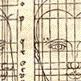
\includegraphics[width=2cm,height=2cm]{./graphics/FF4.jpg}
\end{itemize}
\end{frame}

\section{Useful Hints}

\begin{frame}[fragile]
\frametitle{Useful hints}
\begin{itemize}
\item if you use a verbatim environment on a slide, declare that slide {\tt fragile}:
\begin{verbatim}
\begin{frame}[fragile]
\end{verbatim}
\item bibliography actually works as usual, just keep in mind that not all bibliography styles are supported by the {\it beamer}
      package, maybe you have to include some other packages to get your preferred style working  
\end{itemize}
\end{frame}

\nocite{*}

\begin{frame}[allowframebreaks]
\Large{References} \\[0.5cm]
\tiny
\bibliographystyle{unsrtnat}
\bibliography{./bibliography/LaTeX}
\end{frame} 

\end{document}